\documentclass[12pt]{article}

\usepackage[utf8]{inputenc}
\usepackage[russian]{babel}
\usepackage{graphicx}
\usepackage{indentfirst}
\usepackage{booktabs}
\usepackage{amsmath}


\graphicspath{{pic/}}

\begin{document}

\begin{center}
	\LARGE 
	\textbf{Лабораторная работа 1}\\
	Вычисление определённых интегралов методом Монте-Карло
	\\[3\baselineskip]
\end{center}

\begin{flushright}
	\large
	Выполнил:\\
	студент гр. P4106\\
	Игнашов Иван Максимович\\
	Вариант 8\\
\end{flushright}

\newpage

 \section*{1. Цель работы}
Изучение метода Монте-Карло, определение точности вычисления определенных интегралов методом Монте-Карло.

\subsection*{Порядок работы:}
\begin{enumerate}
	\item Записать математически анализируемую функцию 
		\begin{equation}
			f_{res} = \begin{cases}
						5*sin(2 \pi t) + 1 &t < 1\\
						5*sin(2 \pi (t-1)) + 1 &1 \le t \le 2\\
						2,5* \frac{2}{(t-2) + 1} &t > 2
					  \end{cases}
		\end{equation}
	\item Вычислить аналитически определенный интеграл $F = \int_0^3 f_{res}(t)dt$
	\item Разработать программу, вычисляющую величину F методом Монте-Карло при
заданном числе экспериментов
	\item При помощи разработанной программы вычислить определенный интеграл $\hat{F}$ %$\overset{^}{F}$
 при $N = 2^i$ экспериментах, где i = 0\dots14
\end{enumerate}

\newpage
 \section*{2. График функции $f_{res}(t)$}%
 \begin{figure}[!h]
	\centering
	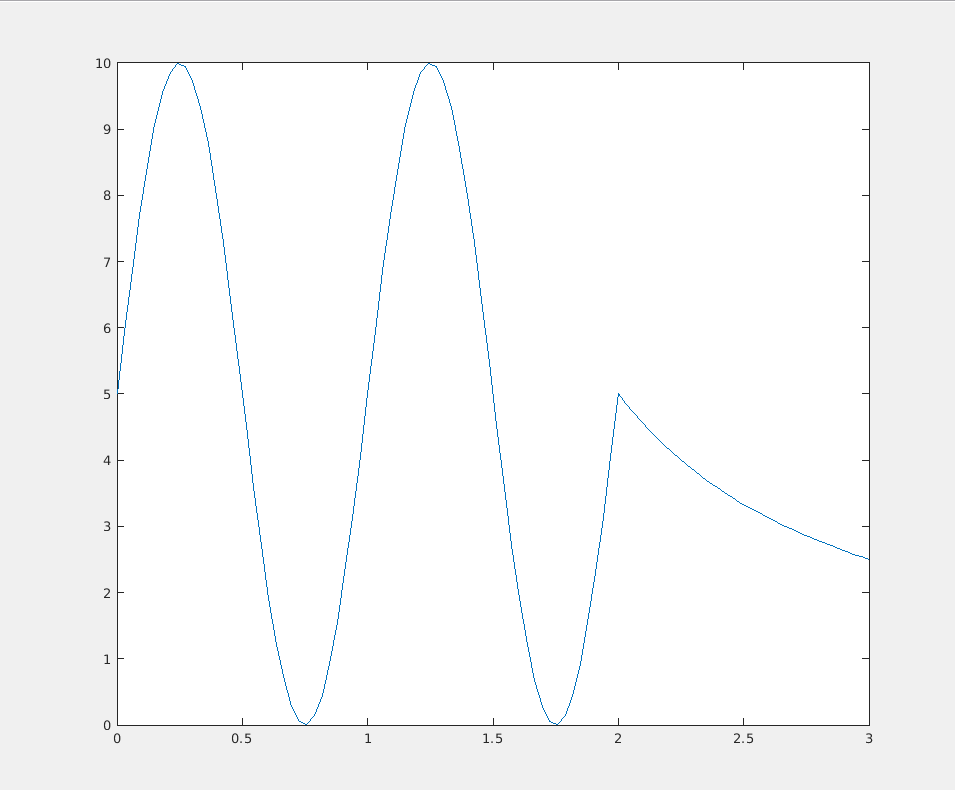
\includegraphics[width=0.5\linewidth]{func_graph.png}
	\caption{График функции $f_{res}(t)$}
\end{figure}
Можно заметить, что на интересующей области $t = [0,3]$ функция принимает значения от 0 до 10
 
 \section*{3. Аналитический расчет величины F}
Проинтегрируем кусочно-заданную функцию отдельно для каждого участка
\begin{center}
	\begin{tabular}[c]{lc|c|c}
  		& $f_1(t)$ & $f_2(t)$ & $f_3(t)$ \\[2mm]\hline
  		&&&\\
		Функция & $5*sin(2 \pi t) + 1$ & $5*sin(2 \pi (t-1)) + 1$ & $2,5* \frac{2}{(t-2) + 1}$\\
		&&&\\
		Неопр. интеграл & $5t - \frac{5cos(2 \pi t)}{2 \pi}$ & $5t - \frac{5cos(2 \pi t)}{2 \pi}$ & $5\log(t-1)$\\
		&&&\\
		Область & $0 \le t \le 1$ & $1 \le t \le 2$ & $2 \le t \le 3$\\
		&&&\\
		Значение & $5.0$ & $5.0$ & $3.46$\\\\
	\end{tabular}
\end{center}

Просуммировав получим $F = 13.46574$
 
\newpage
 \section*{4. Описание разработанной программы}
 %список использованных переменных, блок-схема, текст программы
 
 \begin{figure}[!h]
	\centering
	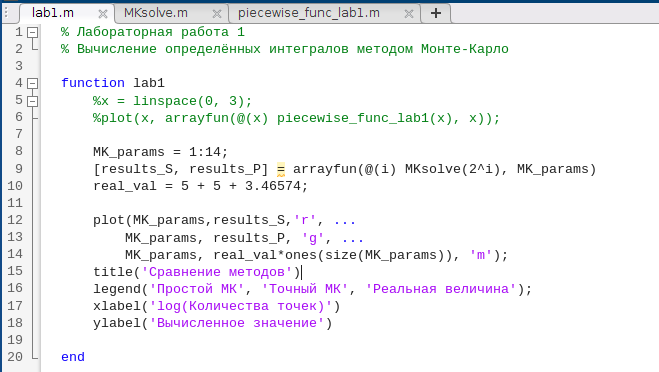
\includegraphics[width=\linewidth]{lab1.png}
	\caption{Код сценария перебора экспериментов}
\end{figure}

Скрипт-сценариий \textbf{\textit{lab1.m}} - точка входа программы, предназначен для запуска всех остальных функции и скриптов, а так же для вывода графика результатов работы.\\

Основные переменные \textbf{\textit{lab1.m}}:
\begin{itemize}
	\item {\textit{results\_S}} - результаты оценки интеграла простым методом Монте-Карло для разных количеств экспериментов
	\item \textit{results\_P} - результаты оценки интеграла методом Монте-Карло с повышенной точностью для разных количеств экспериментов
	\item \textit{real\_val} - реальное значение интеграла
\end{itemize}
 
\begin{figure}[!h]
	\centering
	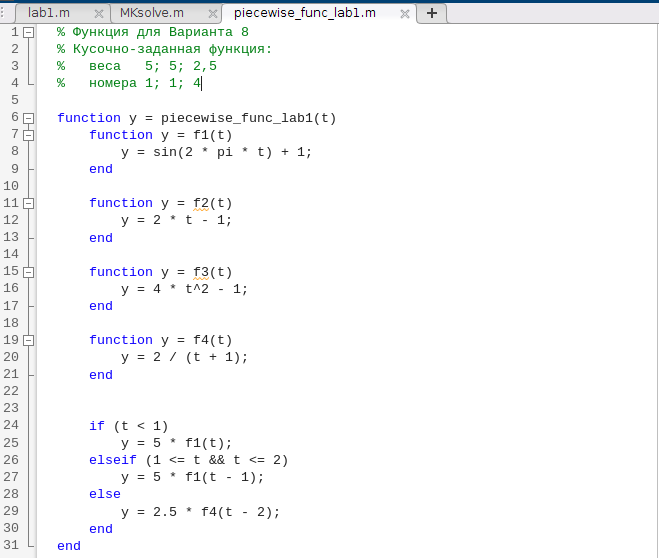
\includegraphics[width=\linewidth]{piecewise_func.png}
	\caption{Код кусочно-заданной функции для Варианта 8}
\end{figure}

\newpage

Скрипт-функция \textbf{\textit{piecewise\_func\_lab1.m}} - записанная в MatLab функция $f_{res}(t)$, интеграл которой и необходимо проанализировать.\\

Основные переменные \textbf{\textit{piecewise\_func\_lab1.m}}:
\begin{itemize}
	\item \textit{f1(t), f2(t), f3(t), f4(t)} - функции расчёта из перечня для вариантов лабораторной работы
\end{itemize}

\newpage
 
\begin{figure}[!h]
	\centering
	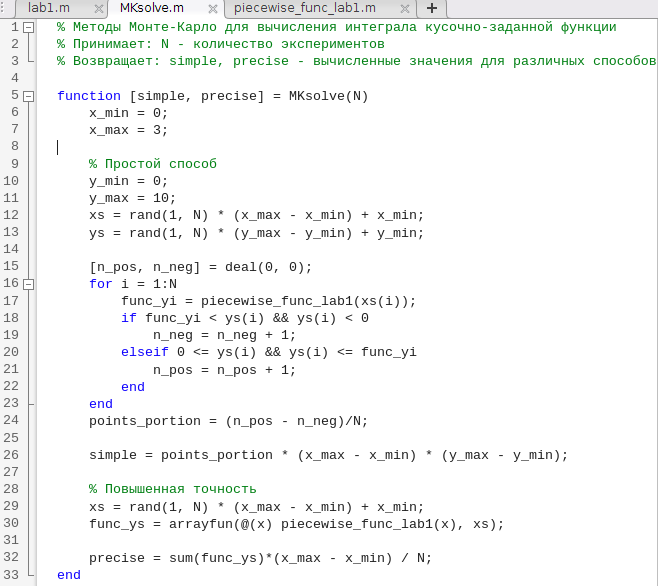
\includegraphics[width=\linewidth]{MKsolve.png}
	\caption{Код функции вычисления интеграла}
\end{figure}

Скрипт-функция \textbf{\textit{MKsolve.m}} - функция реализующая методы Монте-Карло для нахождения интеграла функции \textbf{\textit{piecewise\_func\_lab1}}

Основные переменные \textbf{\textit{MKsolve.m}}:
\begin{itemize}
	\item \textit{[x\_min, x\_max]} - область определения функции $f_{res}$, задаваемая задачей
	\item \textit{[y\_min, y\_max]} - область значений функции $f_{res}$, необходимая для простого метода Монте-Карло
	\item \textit{xs} - случайные точки, сгенерированные равномерным распределением на области определения (используются в обоих методах)
	\item \textit{ys} - случайные значения для точек \textit{xs} в простом методе
	\item \textit{func\_yi} - значение функции $f_{res}$ в точке из \textit{xs}
	\item \textit{simple, precise} - найденные значения интеграла методами "простым" и "более точным" соответственно
\end{itemize}


 \section*{5. Табличное представление результатов моделирования $F(N)$}
 
\begin{figure}[!h]
	\centering
	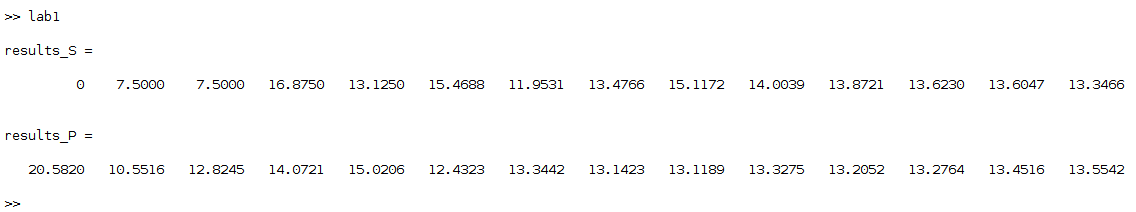
\includegraphics[width=\linewidth]{output.png}
	\caption{Вывод программы}
\end{figure}

\begin{flushleft}

	Получим талицу значений для двух подходов:\\
	\begin{tabular}[c]{c|cc}
		$log_2(N)$ & "Простой" & "Точный" \\
		\hline
		1 & 0.00 & 20.58 \\
		2 & 7.50 & 10.55 \\
		3 & 7.50 & 12.82 \\
		4 & 16.87 & 14.07 \\
		5 & 13.12 & 15.02 \\
		6 & 15.47 & 12.43 \\
		7 & 11.95 & 13.34 \\
		8 & 13.48 & 13.14 \\
		9 & 15.12 & 13.12 \\
		10 & 14.00 & 13.33 \\
		11 & 13.88 & 13.20 \\
		12 & 13.62 & 13.27 \\
		13 & 13.60 & 13.45 \\
		14 & 13.35 & 13.55 \\
	\end{tabular}
	
%	\begin{tabular}[c]{lcccccccccccccc}
		
%  		$2^i$ & 1 & 2 & 3 & 4 & 5 & 6 & 7 & 8 & 9 & 10 & 11 & 12 & 13 & 14\\[2mm]\hline
%  		&&&\\
%		Простой & 0.00 & 7.50 & 7.50 & 16.87 & 13.12 & 15.47 & 11.95 & 13.48 & 15.12 & 14.00 & 13.88 & 13.60 & 13.35\\
%		&&&\\
%		Точный & 20.58 & 10.55 & 12.82 & 14.07 & 15.02 & 12.43 & 13.14 & 13.12 & 13.33 & 13.20 & 13.27 & 13.45 & 13.55\\
%		&&&\\
%	\end{tabular}
\end{flushleft}


\newpage
 \section*{6. График по рассчитанной таблице}
 
\begin{figure}[!h]
	\centering
	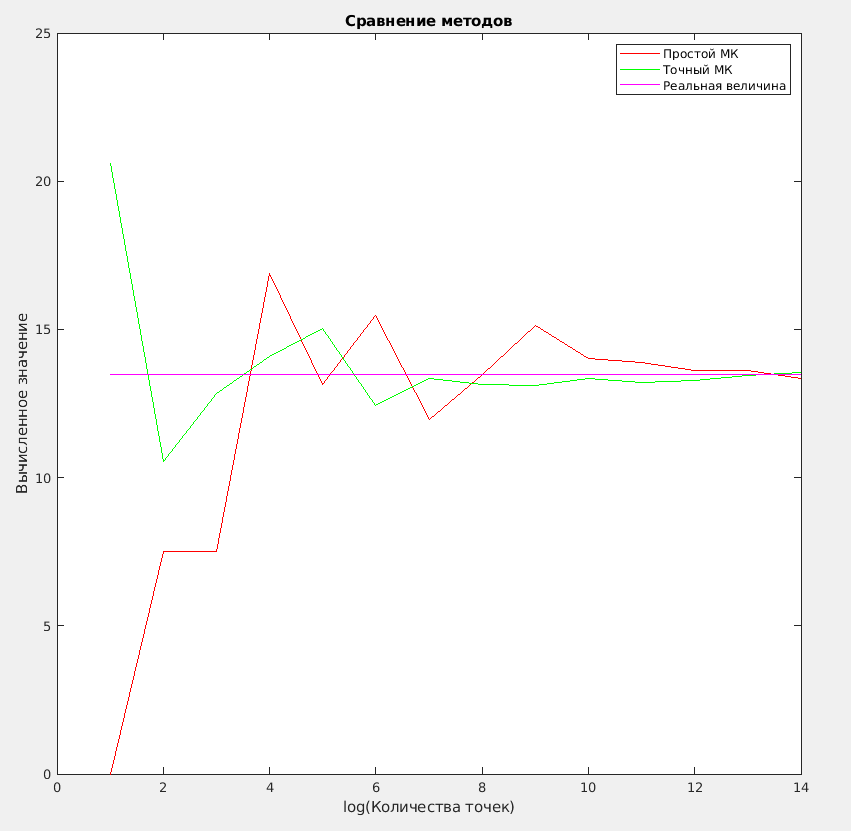
\includegraphics[width=\linewidth]{MK_compare_graph.png}
	\caption{Сравнение графиков методов}
\end{figure}

На графике можно увидеть более быструю сходимость значений точного метода Монте-Карло к реальной величине интеграла


\newpage
 \section*{7. Выводы}
Целью данной лабораторной работы было изучение метода Монте-Карло и его применение. В процессе выполнения были реализованы 2 метода оценки интеграла функции: 

\begin{itemize}
	\item простой - основанный на площадях фигур
	\item с повышенной точностью - вычисление функции на случайных величинах $a_1\dots a_N$
\end{itemize}

На основе вывода программы были получены оценки инеграла функции двумя методами для различного количества случайных точек; построен график сравнения оценок с исходным, вычисленым аналитически, значением интеграла функции.

\end{document}